\documentclass[border=6pt]{standalone}
\usepackage{tikz}
\usetikzlibrary{arrows.meta,positioning,calc,shapes.geometric}
\begin{document}
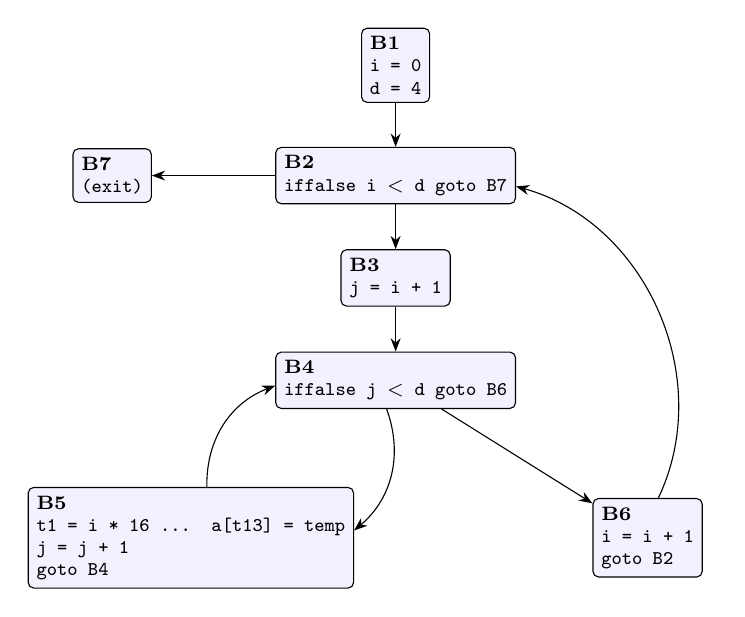
\begin{tikzpicture}[>=Stealth,font=\scriptsize,x=1.000cm,y=1.000cm,
 box/.style={draw,rounded corners=2pt,align=left,inner sep=3pt,fill=blue!5},
 circ/.style={draw,circle,align=center,inner sep=1pt,minimum size=0.75cm,fill=blue!5},
 lab/.style={font=\scriptsize,inner sep=1pt,fill=white,fill opacity=0.85,text opacity=1}]
\node[box] (b1) at (0.000,0.000) {\textbf{B1}\\\texttt{i = 0}\\\texttt{d = 4}};
\node[box] (b2) at (0.000,-1.400) {\textbf{B2}\\\texttt{iffalse i \textless{} d goto B7}};
\node[box] (b3) at (0.000,-2.700) {\textbf{B3}\\\texttt{j = i + 1}};
\node[box] (b4) at (0.000,-4.000) {\textbf{B4}\\\texttt{iffalse j \textless{} d goto B6}};
\node[box] (b5) at (-2.600,-6.000) {\textbf{B5}\\\texttt{t1 = i * 16 ... a[t13] = temp}\\\texttt{j = j + 1}\\\texttt{goto B4}};
\node[box] (b6) at (3.200,-6.000) {\textbf{B6}\\\texttt{i = i + 1}\\\texttt{goto B2}};
\node[box] (b7) at (-3.600,-1.400) {\textbf{B7}\\\texttt{(exit)}};
\draw[->] (b1) --  (b2);
\draw[->] (b2) --  (b3);
\draw[->] (b2) --  (b7);
\draw[->] (b3) --  (b4);
\draw[->] (b4) to[bend left=35]  (b5);
\draw[->] (b4) --  (b6);
\draw[->] (b5) to[bend left=35]  (b4);
\draw[->] (b6) to[bend right=50]  (b2);
\end{tikzpicture}
\end{document}
